\documentclass[12pt,twoside,english,a4paper]{article}

\usepackage[english]{babel}
\usepackage[IL2]{fontenc} % lepšia sadzba písmena Ľ než v T1
\usepackage[utf8]{inputenc}
\usepackage{graphicx}
\usepackage{url} % príkaz \url na formátovanie URL
\usepackage{hyperref} % odkazy v texte budú aktívne (pri niektorých triedach dokumentov spôsobuje posun textu)

\usepackage{cite}
%\usepackage{times}

\pagestyle{headings}

\title{FOOTBALL SIMULATORS (FIFA AND PES)}

\author{Dmytro Barninets\\[2pt]
	{\small Slovenská technická univerzita v Bratislave}\\
	{\small Fakulta informatiky a informačných technológií}\\
	{\large \texttt{xbarninets@stuba.sk}}
	}

\date{\large 11. october 2022}



\begin{document}

\maketitle


\section{Why did i chose this topic?} \label{mainparagraph}

The main reason I chose this theme is the popularity of football games. Among sports simulators, it is FIFA that occupies a leading position in online.


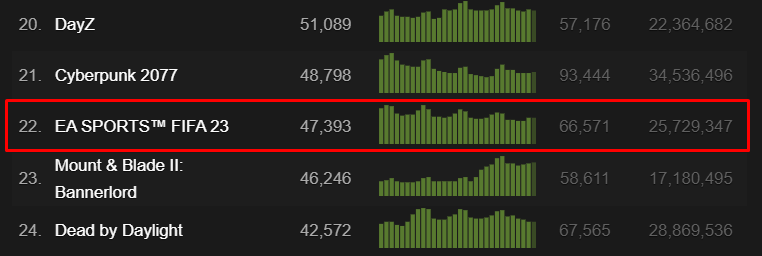
\includegraphics[width=150mm,scale=1.5]{fifa_charts.png} \label{chartsphoto}


As of November 4, an average of 47,000 players play FIFA. And this is only in Steam, excluding consoles and less popular game launchers.


As for PES, the situation with online is much worse at the moment \emph{(more on that later)}. But that doesn't stop footsim fans from remembering this series as legendary.

In general, football simulators are not as simple and monotonous as at first glance.

\section{Differences between FIFA and PES} \label{differences}\cite{Gaming.net}

\begin{itemize}
\item What is FIFA?

FIFA is a video game series that is published by Electronic Arts (EA) and developed by EA Canada.

From the very first versions FIFA obtained more licenses in comparison to their rivals. The licenses obtained include permits for stadiums, players and their respective clubs. This helps guarantee the production of realistic football games; since users prefer playing with real characters, they are familiar with and can relate to. That and various other aspects are what make FIFA a remarkable series. In terms of sales, FIFA is ahead of PES, although the latter has always been regarded as the better game. Nonetheless, it may still have a long way to go before it achieves the same commercial effect as FIFA.

\item What is PES?

Pro Evolution Soccer [PES] is a video game series that is published by Konami and developed by PES Productions. PES games are released annually, with the latest one being PES 2021. 

Much like FIFA, PES aspires to be as realistic as possible when it comes to depicting real-life football. Hence, the gameplay in its series is identical to association soccer, whereby players control either one player or a whole team. The ideas of the game also correspond with the rules and regulations of the football association.
	
\end{itemize}

The most apparent difference between the two game brands is the time gap between the first launch of PES’s first game and that of FIFA. This gave FIFA a chance to fully develop a fan base and perfect its products over the years. 

However, PES was able to compete as they adopted much more diverse models in their gameplay compared to FIFA. Similarly, in terms of gameplay, most fans regard PES as more practical, whilst FIFA is considered more refined in design and presentation. 



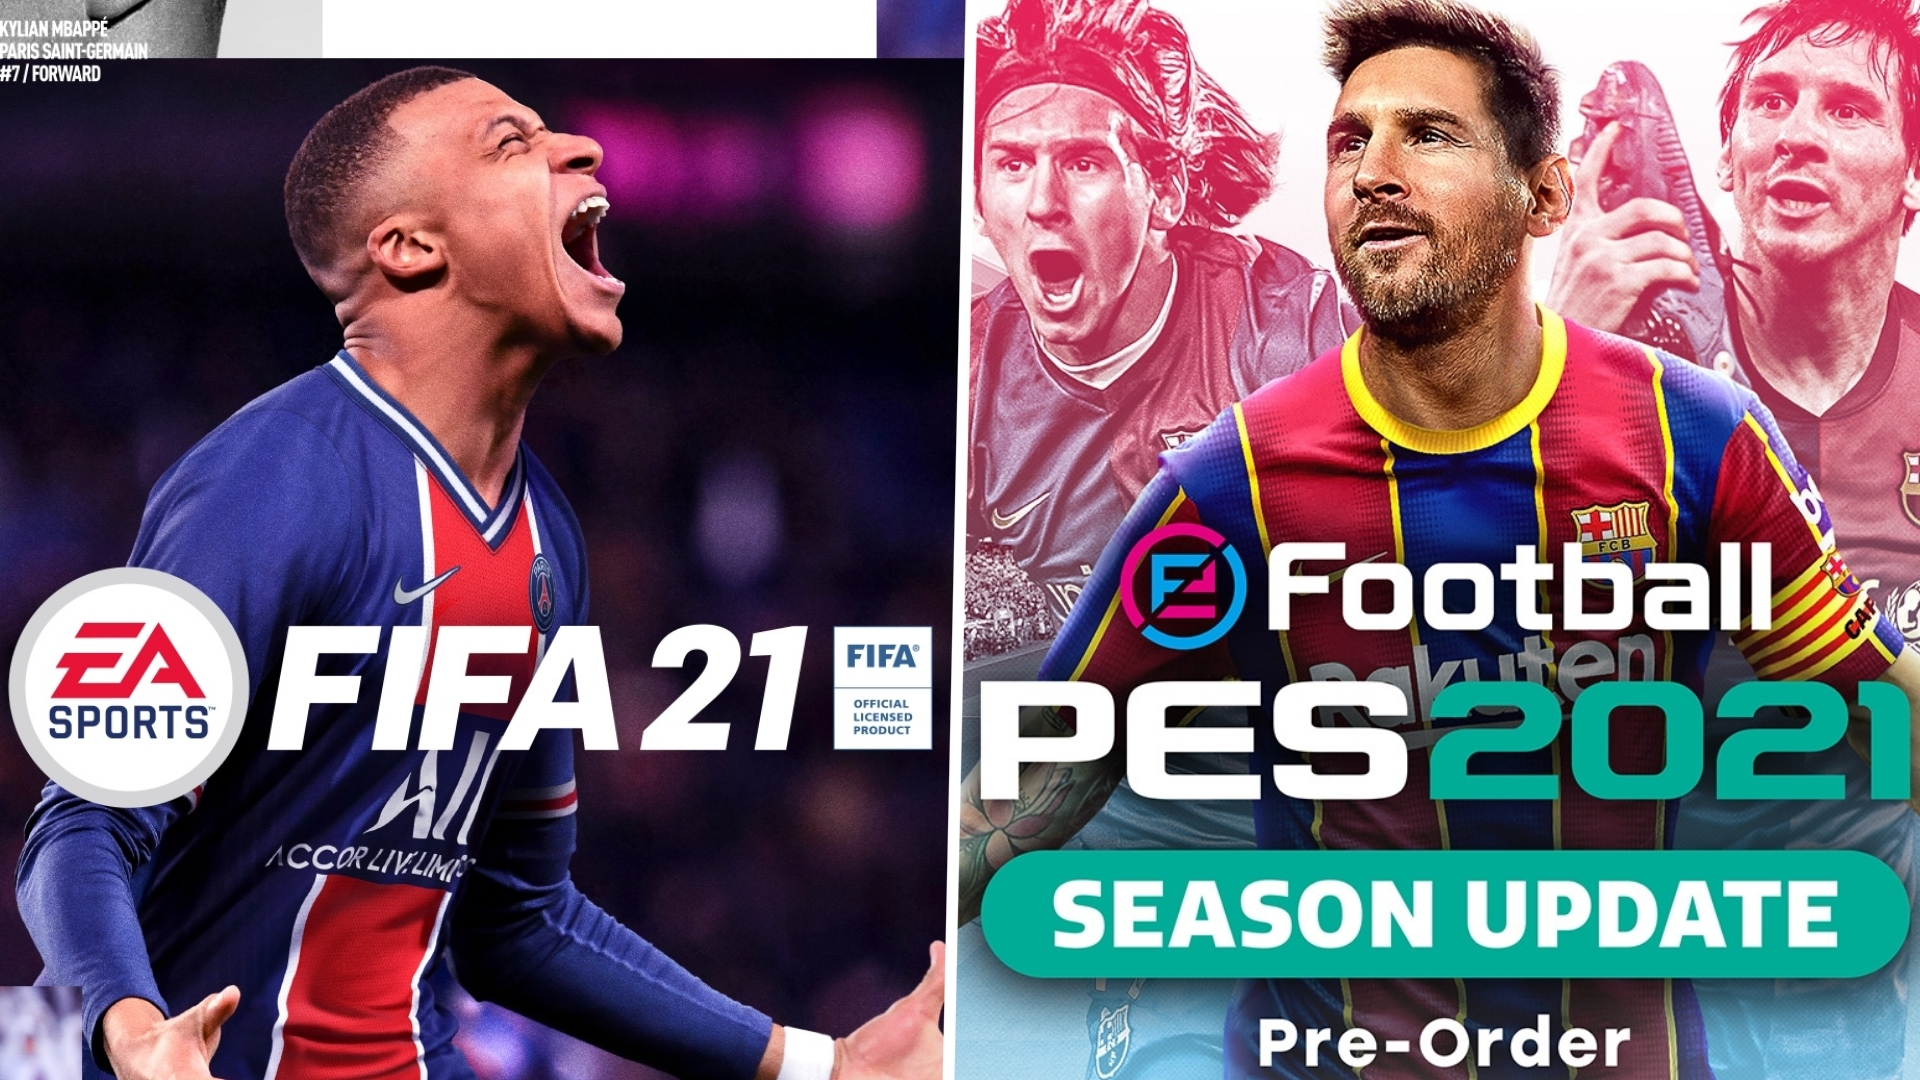
\includegraphics[width=150mm,scale=1.5]{fifaandpes.jpeg} \label{fifaandpes}


\section{Game aspects} \label{aspects}




\subsection{Graphics} \label{aspects: graphics}
This is one of the most noticeable differences between FIFA and PES. FIFA’s graphics have been consistently better than PES’s for a few years now. FIFA’s player models look more realistic and the stadiums are more accurately recreated in FIFA games. PES’s graphics have improved in recent years, but they still don’t match up to FIFA’s.

\subsubsection{Engines}

We know that PES will be using the Unreal Engine produced by Epic Games. While Unreal Engine is due towards the end of 2021, eFootball will use Unreal Engine 4, which still will see some major enhancements from a graphical perspective.

FIFA will continue running on the Frostbite engine, so we can probably expect more iterative improvements. It is generally regarded as the prettier, more polished game. So it will be interesting to see how they both look in the 2022 editions.

\subsection{Gameplay} \label{aspects: gameplay}
The gameplay is where PES really excels. PES games have always had great gameplay, with players feeling more responsive and the controls feeling tighter than FIFA’s.

\subsection{Game modes} \label{aspects: modes}
FIFA games have always had more features than PES games. The Career modes such as the Europa League and Champions League featured by FIFA have the liberty to be as authentic as possible with their gameplay.

Other various modes provided in FIFA games include Career Mode, Volta, Ultimate Team and Manager Mode. On the other hand, we have PES making the best of its various but limited modes which include Master League and myClub, which is the equivalent of FIFA’s Ultimate Team mode.

\subsection{Teams} \label{aspects: teams}
For a long time, FIFA has enjoyed a monopoly in terms of real players, teams and stadiums. This has been a big factor in enhancing the game’s realism in a way that PES is still trying to measure up to. They have unlimited access to players, logos and teams, making it easier to replicate the most realistic games possible. Hopefully, PES will be able to do the same, thanks to Juventus and various other teams who intend to exclusively grant them a license. Nonetheless, in this category, FIFA remains dominant.

\subsection{Players} \label{aspects: players}
For PES, the player rosters are not as complete as players would wish them to be; these constraints not only go beyond teams but with players as well. However, PES has made progress in acquiring significant players like Messi so far, such that players will not experience as much difficulty when playing major leagues using international teams. As for FIFA, their advantage is apparent as all the divisions of players and their teams are accounted for. \cite{Stealthoptional.com}

\section{History} \label{history}
Clearly, FIFA is the bigger franchise. In terms of pure sales, it ranks somewhere in the region of series like Call of Duty and Grand Theft Auto, which are no joke. PES is still a massive seller with over 100 million units, making it comparable to the likes of The Legend of Zelda and Resident Evil in volume.

The lack of licensed players, teams, and stadia seems to have done irreparable damage to the Konami series, though. No matter how much you like the arcade-style gameplay of PES, it's meant to be a simulation game, and a massive part of that is getting to play as your favourite teams and players.

However, as we fast approach the 2022 versions of these football titles, it seems the two titans will now go in slightly different directions.

PES 2022, as it would have been known, won't really exist. Konami has announced the rebranding of PES simply to eFootball, following the previous rebranding to eFootball PES a few years ago. Aside from this, eFootball will be a free-to-play title, signalling Konami's intention to monetise their football game differently than previous titles, and FIFA 22.

Maybe this will see eFootball/PES finally catch up to FIFA in sales?

Niekedy treba uviesť zoznam:




\bibliography{literatura}
\bibliographystyle{plain}
\end{document}
